\section{How to cite}
Use \textbf{parencite} to do a standard citation, e.g. \parencite{Elliott2016}. Each chapter in this thesis template is self-contained in that each chapter has its own bibliography. 

\section{Glossary}
Optional. You can add entries into \textbf{frontmatter/glossary.tex}. Each entry must be referenced at least once using the \textbf{gls} command. Here's an example:

I want the word `\gls{climate model}' in the glossary.

\begin{figure}
    \centering
    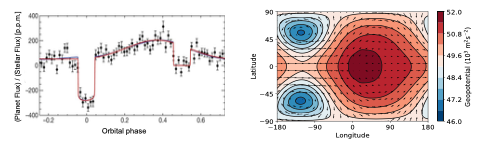
\includegraphics{figures/random-figure.png}
    \caption{Caption}
    \label{fig:my_label}
\end{figure}

\section{Acronyms}
Same as above. Entries added into \textbf{frontmatter/acronyms.tex}. An example: the \acrlong{ipcc} can be input in long-form or short-form \acrshort{ipcc}.